% colors for code highlighting
\definecolor{mygreen}{RGB}{28,172,0}
\definecolor{mylilas}{RGB}{170,55,241}
\definecolor{deepblue}{rgb}{0,0,0.5}
\definecolor{deepred}{rgb}{0.6,0,0}
\definecolor{deepgreen}{rgb}{0,0.5,0}
\definecolor{lightgray}{rgb}{0.6,0.6,0.6}

% julia langage definition
\lstdefinelanguage{Julia}%
  {morekeywords={abstract,break,case,catch,const,continue,do,else,elseif,%
      end,export,false,for,function,immutable,import,importall,if,in,%
      macro,module,otherwise,quote,return,struct,switch,true,try,type,typealias,%
      using,while},%
   sensitive=true,%
   alsoother={\$,<:,::},%
   morecomment=[l]\#,%
   morecomment=[n]{\#=}{=\#},%
   morestring=[s]{"}{"},%
   morestring=[m]{'}{'},%
}[keywords,comments,strings]%

% general parameters for listings
\lstset{%
    breaklines          = true, %
    showstringspaces    = false,%
    basicstyle          = \ttfamily\small,
    inputencoding=utf8,
    extendedchars=true,
    % numbers=left, %
    % numberstyle={\tiny \color{black}},%
    frame               = leftline,%
    basewidth           = 0.45em,%
}
% MATLAB
\newcommand\matlabstyle{\lstset{%
    language=Matlab,%
    keywordstyle=\color{blue},%
    stringstyle=\color{mylilas},%
    commentstyle=\color{mygreen},%
    numberstyle={\small \color{black}},%
    numbersep=10pt, % 
    emph=[1]{classdef, for,end,break},emphstyle=[1]\color{red},%
}}
% PYTHON
\newcommand\pythonstyle{\lstset{%
    language=Python,%
    keywordstyle=\color{deepblue},%
    stringstyle=\color{deepgreen},%
    commentstyle=\color{lightgray},%
    otherkeywords={self},
}}
% JULIA
\newcommand\juliastyle{\lstset{%
    language         = Julia,
    keywordstyle     = \bfseries\color{blue},
    stringstyle      = \color{magenta},
    commentstyle     = \color{ForestGreen},
}}



% http://wiki.ljp.upmc.fr/zebrain/
% analyse en Julia




\chapter{Outils informatiques}\label{AppA}

\section{Simulation de l'effet de lentille thermique}\label{APPsimuthermallens}

Le code de cette simulation numérique est publié à l'adresse :
\\ \href{https://github.com/Hugo-Trentesaux/these}{https://github.com/Hugo-Trentesaux/these}.
J'en décris ici le fonctionnement général.

Le fichier \verb|gaussianbeam.jl| contient les fonctions relatives à la propagation d'un faisceau gaussien. Le fichier \verb|grinlens.jl| contient le modèle proprement dit, il définit deux structures (\verb|Parameters| et \verb|Observables|) et une fonction (\verb|propagate|). La structure \verb|Parameters| contient les paramètres de la simulation, la structure \verb|Observables| contient une trace des différentes variables observables tout au long de la simulation. La fonction \verb|propagate| applique la formule des lentilles gaussiennes en itérant sur les lentilles fines successives. Des portions de code sont masquées et remplacées par \verb|[...]| pour plus de lisibilité (attention, un bug étrange dans \LaTeX déplace certains caractères unicode).

\juliastyle
\begin{lstlisting}
# [...] module stuff

# parameters
Base.@kwdef struct Parameters
    # medium parameters
    n       # index of refraction
    lλ       # wavelength (m)
    P       # power of laser (W)
    k       # thermic diffusion coefficient (W/m/K)
    aα       # absorption coefficient (1/m)
    dndT    # index variation coefficient (1/K)
    focale::Function  # thermally induced focal length of liquid slice

    # input beam parameters    
    z0      # initial position of the waist without lens effect (m)
    w0      # initial waist of the beam (m)
    
    # iteration parameters
    l       # width of the liquid slices (m)
    steps   # position along the tank to compute on (m)
end

# [...] default parameters
   
# observables
mutable struct Observables
    focal::Vector   # focal length of liquid slice lens (m)
    shift::Vector   # focal shift generated by liquid slice lens (m)
    magnif::Vector  # magnification for liquid slice lens 
    pos::Vector     # position of the waist after liquid slice lens (m)
    waist::Vector   # size of the waist after liquid slice lens (m)
    wonlens::Vector # beam width on the lens (m)
    dist::Vector    # distance from lens to object waist (m)
    minwidth        # minimal width of the beam (m)
    minwidthpos     # first position of minimal width (m)
end

# simulate a gaussian beam propagation in water
function propagate(n,lλ,focale,z0,w0,l,steps)
    # observables
    o = Observables(length(steps))   # initialize observables

    # loop for each element lens
    for (i,z) in enumerate(steps)        
        # compute lens effect
        sa = z0 - z                         # algebric distance lens-object
        w0a = w0                            # waist before lens
        zra = rayleigh_length(n, w0a, λ)    # Rayleigh length before lens
        wa = gaussian_width(n, sa, w0a, λ)  # beam width at lens position
        fprime = focale(l, wa)              # thermally induced focal length
        sb = sprime(sa, fprime, zra)        # algebric distance lens-image
        mag = magnification(sa, fprime, zra) # magnification
        w0b = w0a * mag                     # waist after lens

        # update beam properties
        z0 = z + sb                         # update z0 with new beam position
        w0 = w0b                            # update w0 with new beam waist

        # [...] update observables
    end
    (o.minwidth, pos) = findmin(o.wonlens)  # get minimal width and its position
    o.minwidthpos = steps[pos]            # convert it to meter
    return o
end

# [...]
\end{lstlisting}

Ensuite, il suffit de définir des paramètres déclarant les valeurs différentes de celles par défaut, d'appeler la fonction \verb|propagate|, et d'afficher les observables dans une figure. Le fichier \verb|grinlensplots_these.jl| contient le code ayant servi à générer les figures de ce manuscrit concernant la simulation. Voici en exemple une figure bonus :

\juliastyle
\begin{lstlisting}
pows = 0:0.01:1     # power range for waist magnification
# vector of parameters for these values of power
P = map(p -> Parameters(P=p, l=1e-6, w0=4e-6, n=1.33), pows)
O = propagate.(P) # apply propagation on each parameter

minwidth = map(o->o.minwidth, O).*1e3 # select minwidth observable
plot(pows, pows./minwidth.^2, lw=3, size=(600,400), legend=false,
    gridlinewidth=3, thickness_scaling=1.5) # plot it
xlabel!("puissance laser (W)")
ylabel!("intensité maximale (W/mm²)")
savefig("grinlensplots_these_maxpower.png")
\end{lstlisting}

\begin{figure}
    \centering
    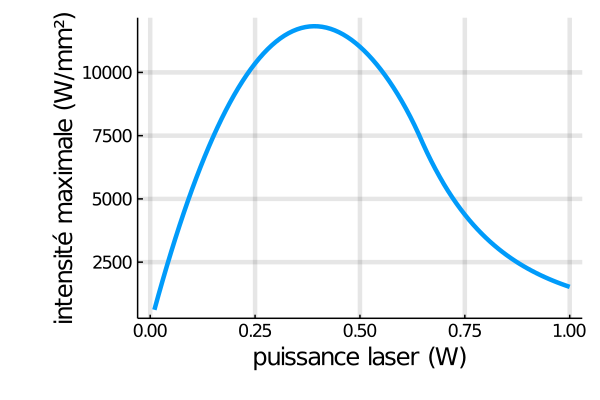
\includegraphics[width=0.6\textwidth]{./files/grinlensplots_these_maxpower.png}
    \caption{Intensité maximale du faisceau en fonction de la puissance laser. Dans un premier temps, augmenter la puissance laser augmente la puissance maximale, mais dans un deuxième temps, la puissance maximale diminue à cause de l'élargissement du faisceau.
    \label{AppFIGmaxintensity}}
    \end{figure}


\section{Langage de programmation adapté}

\subsection{Memory mapping}

Du fait du volume des données traitées, notre processus d'analyse repose largement sur le \verb|memory mapping| comme solution de gestion des données brutes. Cela permet de traiter une portion de mémoire disque comme une portion de mémoire vive et ainsi de n'appliquer les opérations de chargement de données en mémoire vive qu'au moment de leur utilisation et de ne pas écrire systématiquement les opérations de lecture et d'écriture. Je compare ici les interfaces fournies dans les langages de programmation Matlab, Python, et Julia ainsi que la manière dont elles peuvent être étendues par des classes ou structures.

\subsubsection{Matlab}

La langage Matlab fournit la fonction \verb|memmapfile| (\href{https://fr.mathworks.com/help/matlab/ref/memmapfile.html}{doc}) qui permet de cartographier une zone mémoire contenant des données de type \verb|int8|, \verb|int16|, \verb|int32|, \verb|int64|, \verb|uint8|, \verb|uint16|, \verb|uint32|, \verb|uint64|, \verb|single|, ou \verb|double|.
J'ai implémenté plusieurs surcouches de la classe Matlab \verb|memmapfile| qui permettent de gérer l'accès à des données stockées sous différents formats comme le \verb|dcimg|, d'autres orientations que celle par défaut, et en utilisant l'indexation linéaire suivant (xy) en une seule ligne. Ces classes ont facilité l'écriture de code pour la manipulation des données brutes et aux différentes étapes de traitement, ainsi que des interfaces graphiques rudimentaires utilisées pour les visualiser mais ne permettent pas de profiter des optimisations de Matlab sur la vectorisation du calcul.
De plus, une gestion manuelle de la mémoire et des abstractions sur les tableaux de données manquent au langage pour que ces classes soit facilement réutilisables, ce qui conduit à de la duplication de code. Ci-dessous on peut voir la structure adoptée pour ces classes, qui surchargent les méthodes intégrées au langage \verb|subsref| et \verb|subsasgn|.


\matlabstyle
\begin{lstlisting}
classdef Mmap < handle
% the class Mmap is used to load a mmap of a binary file
% and redefine layers index when called as subscript
% subscript can be 4D or 3D

% [...] properties, contructor, and other methods definition

function out = subsref(self, S)        
    switch S(1).type
        case '()'
            new_S = self.subStruct(S);
            % [...] subscript manipulation
            out = subsref(self.mmap.Data.bit, new_S);
            % [...] returned data manipulation
            end
        case '.'
            out = builtin('subsref', self, S);
        otherwise
            error('subsref other than () or . not implemented')
    end        
end

end
\end{lstlisting}

\subsubsection{Python}

Le langage Python offre également une classe \verb|mmap| (\href{https://docs.python.org/3.8/library/mmap.html}{doc}) ainsi que sa bibliothèque Numpy avec la classe \verb|memmap| (\href{https://numpy.org/devdocs/reference/generated/numpy.memmap.html}{doc}). Une option \verb|order| permet de préciser l'ordre des données en mémoire, et donc d'adapter simplement la manière dont les données sont stockées à la manière donc elles seront utilisées. CaImAn implémente également une surcouche fine sur cette classe pour gérer ses conventions d'organisation de fichiers, où de nombreuses informations sont contenues dans le nom de fichier. J'en montre ci-dessous un extrait.

\pythonstyle
\begin{lstlisting}
def load_memmap(filename: str, mode: str = 'r') ->
    Tuple[Any, Tuple, int]:
    # [...]
    Yr = np.memmap(
        file_to_load,
        mode=mode,
        shape=prepare_shape((d1 * d2 * d3, T)),
        dtype=np.float32,
        order=order
        )
    if d3 == 1:
        return (Yr, (d1, d2), T)
    else:
        return (Yr, (d1, d2, d3), T)
\end{lstlisting}


\subsubsection{Julia}

Le langage Julia intègre un module dédié au \verb|memory mapping| (\href{https://docs.julialang.org/en/v1/stdlib/Mmap/index.html#Mmap.mmap}{doc}) qui permet d'accéder aux données par un objet qui se comporte de manière identique à un tableau Julia. Via le concept d'interfaces (\href{https://docs.julialang.org/en/v1/manual/interfaces/#man-interface-array-1}{doc}), en particulier l'interface de tableau, il est facile d'écrire une surcouche immédiatement compatible avec n'importe quelle fonction prenant en argument un tableau Julia. Cela est très différent de Matlab où il faut écrire des fonctions spécifiques et légèrement différent de Python où l'écriture de classes intermédiaires génère un surcoût important par rapport à Numpy. Je montre ici un exemple de surcouche mince sur la structure Julia \verb|mmap|.
Il est extrêmement facile de surcharger une telle classe Julia pour l'adapter à des usages différents sans avoir à en modifier le comportement. Par exemple, il suffit d'une dizaine de lignes pour rendre une telle structure compatible avec les données stockées sous le format de CaImAn tout en conservant la compatibilité avec d'autres formats, et pour un coût nul à l'exécution.
% Grâces aux interfaces, à la surcharge de méthodes, au filtrage par motif (\emph{pattern matching}, il est extrêmement facile de surcharger les méthodes d'une classe Julia pour l'adapter à des usages différents sans avoir à en modifier le comportement. Cela offre une souplesse précieuse lors du prototypage de même qu'en production dans des environnements différents. Par exemple, il suffit d'une dizaine de lignes pour rendre une telle structure compatible avec les données stockées sous le format de CaImAn tout en conservant la compatibilité avec d'autres formats, et pour un coût nul à l'exécution.

\juliastyle
\begin{lstlisting}
using Mmap

# ===== structure definition =====
struct Stack{T,N} <: AbstractArray{T,N}
    file::String        # path plus filename of raw raster file
    dims::NTuple{N,Int} # N integers correspondig to dimension sizes
    space::String       # e.g. RAST
    m::Array{T,N}       # memory mapped array
    # core constructor
    Stack(file::String, T::DataType, dims::NTuple, space::String) =
      new{T,length(dims)}(file, dims, space,
        Mmap.mmap(open(file), Array{T, length(dims)}, dims))
end

# [...] more methods like constructor overload

# ===== interface implementation =====
# following functions allows to access Stack like an Array
Base.size(S::Stack) = S.dims
# linear indexing
Base.getindex(S::Stack, i::Int) = S.m[i] 
# cartesian indexing
Base.getindex(S::Stack{T,N}, I::Vararg{Int, N}) where {T,N} = S.m[I...]
\end{lstlisting}


% \subsection{Vitesse d'exécution}
% \subsection{Gestion et maintenance du code}



\subsection{Function broadcasting}

Les langages destinés à traiter des données matricielles peuvent exposer certaines fonctionnalités qui réduisent considérablement le nombre de lignes à écrire. Cependant, toutes ne sont pas égales.

\subsubsection{Matlab}

Si la plupart des fonctions Matlab acceptent des matrices en entrée, cela ne s'applique pas aux matrices stockées par \verb|memory mapping|. De plus, adapter une fonction scalaire en fonction matricielle peut nécessiter une ré-écriture et aboutir à des erreurs difficiles à identifier.

% https://fr.mathworks.com/help/coder/ug/what-are-column-major-and-row-major-representation-1.html

\matlabstyle
\begin{lstlisting}
% define a scalar function
f = @(x) x^2 + 1;
% call it on a scalar (should not call it on a matrix)
f(2) % returns 5
% define an equivalent matrix function using dot operator
F = @(X) X.^2 + 1;
% call it on a matrix
A = [ 1 2 3 ; 2 6 7 ];
F(A) % returns [2 5 10 ; 5 37 50]

% write A to a binary file and use memmapfile to map it
fid = fopen("A.raw", "w"); write(fid, A, "double"); fclose(fid);
m = memmapfile("A.raw", "Format", {"double", [2 3], "bit"});
% can not apply F on it, forced to load data then apply it
F(m) % ERROR Operator '.^' is not supported for operands of type 'memmapfile'.
% must load entirely the matrix which defeats the point of memory mapping
A = m.Data.bit; % copies all values in memory
F(A) % returns the good result

% an other function example not designed for matrix usage
substract_mean_add_first = @(X) X - mean(X) + X(1);
% if we want to transform each row with the "substract_mean_add_first" function
% without rewriting it or changing it, we have to iterate manually
% (here it is not optimal since Matlab has "column-major layout by default")
for i = 1:size(A,1)
    A(i,:) = substract_mean_add_first(A(i,:));
end
% A = [0 1 2; -1 3 4]
\end{lstlisting}

\subsubsection{Python}

En Python, Numpy pratique le \verb|broadcasting| sur les opérateurs élémentaires. Une fonction utilisant ces opérateurs élémentaires peut donc être appliquée sur un \verb|array| Numpy. Cela fonctionne également sur une matrice en \verb|memory mapping|.

\pythonstyle
\begin{lstlisting}
import numpy

# define function
f = lambda x: x**2 +1
f(2) # f can be called on a scalar
A = numpy.array([[1,2,3],[2,6,7]])
f(A) # f can be called on a numpy array

# create memory map
m = numpy.memmap("A.raw", dtype='float64', mode='w+', shape=(2,3), order='F')
m[:] = A[:] # fills it with values of A
m.flush()	# flush to write to disk
f(m) # f can be called on memory map, it returns:
# array([[ 2.,  5., 10.],
#        [17., 26., 50.]])

# example of function applying onto vector
substract_mean_add_first = lambda X: X - numpy.mean(X) + X[0]
# a version of this function that performs in-place modification
def substract_mean_add_first_modif(vector):
	vector[:] = substract_mean_add_first(vector)
	vector.flush() # only for memory mapping
# we can iterate automatically on m to transform its rows
# (order was set to 'F' = row major, which is optimal in this case)
map(substract_mean_add_first_modif, m)
# now m equals :
# memmap([[ 0.,  1.,  2.],
#         [-1.,  3.,  4.]])
\end{lstlisting}

\subsubsection{Julia}

En Julia, le \verb|broadcasting| peut être réalisé sur n'importe quelle fonction ou opérateur en utilisant l'opérateur \verb|dot|. Ainsi, on peut écrire une fonction acceptant une matrice entière en utilisant les opérateurs élément par élément, mais on peut aussi écrire une fonction n'acceptant qu'un scalaire et l'appliquer sur une matrice en utilisant l'opérateur \verb|dot|. C'est une fonctionnalité clé du langage et les performances dépassent systématiquement les autres langages (\href{https://julialang.org/benchmarks/}{benchmarks}).

\juliastyle
\begin{lstlisting}
using Mmap # for memory mapping
using Statistics # for mean

# define function that can only be called on a scalar
f(x::Number) = x^2 + 1
f(2) # f can be called on a scalar
A = [1 2 3; 2 6 7]
f.(A) # f can be called on each element of A thanks to dot broadcasting
# alternatively, we can define a vector matrix version of the function
F(X::Matrix) = X.^2 .+ 1 # it uses the dot operators internally

# create memory mapped file for A
file = open("A.raw", "w+")
m = Mmap.mmap(file, Matrix{Float64}, (2,3)
m[:] = A[:]
f.(m) # f can be broadcasted to m as well

# other function example
substract_mean_add_first(v::AbstractVector) = v .- mean(v) .+ v[1]
# in-place version of this function (julia convention is to end with '!')
function substract_mean_add_first!(v::AbstractVector)
	v[:] = substract_mean_add_first(v)
end
# iterate on each row
map(substract_mean_add_first!, eachrow(m))
# now m equals
# 2×3 Array{Float64,2}:
#   0.0  1.0  2.0
#  -1.0  3.0  4.0
\end{lstlisting}



\section{Atlas interactifs}

Plusieurs outils ont été développés pour explorer le cerveau de poisson zèbre directement dans le navigateur. Je décris rapidement les principaux et en introduis un nouveau que j'ai réalisé pour répondre à certains besoins.

% TODOcite Randlett Tabor Kunst

\subsection{ZBrainAtlas}

Le \href{https://engertlab.fas.harvard.edu/Z-Brain/home/}{Z Brain Atlas} permet de visualiser dans un même espace de référence les tranches horizontales de cerveaux marqués avec des anticorps différents et de superposer les contours de régions anatomiques. Cela permet de parcourir rapidement les différents types de neurones présents dans une certaine zone.

\subsection{MapZebrain}

Le \href{https://fishatlas.neuro.mpg.de/}{Max Planck Zebrafish Brain Atlas} propose trois outils très riches en fonctionnalités pour explorer le cerveau à travers une vue tridimensionnelle. Cette vue peut être en 3D réelle avec perspective avec un angle de vue réglable, en tranche suivant trois plans (sagittal, frontal, transverse), ou en projection isométrique autour de l'axe rostro-caudal.
L'un permet de visualiser les régions anatomiques du cerveau sélectionnées dans une arborescence, ce qui permet de se représenter leur structure tridimensionnelle et leur positions relatives.
Un autre permet de sélectionner la structure tridimensionnelle de neurones uniques filtrés suivant la position du soma, les régions traversées, ou leur position terminale. Un troisième permet de superposer dans plusieurs canaux de couleur les images matricielles correspondant à des cerveaux marqués pour différents cibles.

\subsection{FishExplorer}

Le \href{https://zebrafishatlas.zib.de/}{Fish Explorer} tente de présenter les mêmes données à travers une autre interface. Il n'apporte rien de nouveau pour l'instant.

\subsection{LJPzebrain}

\begin{figure}
\centering
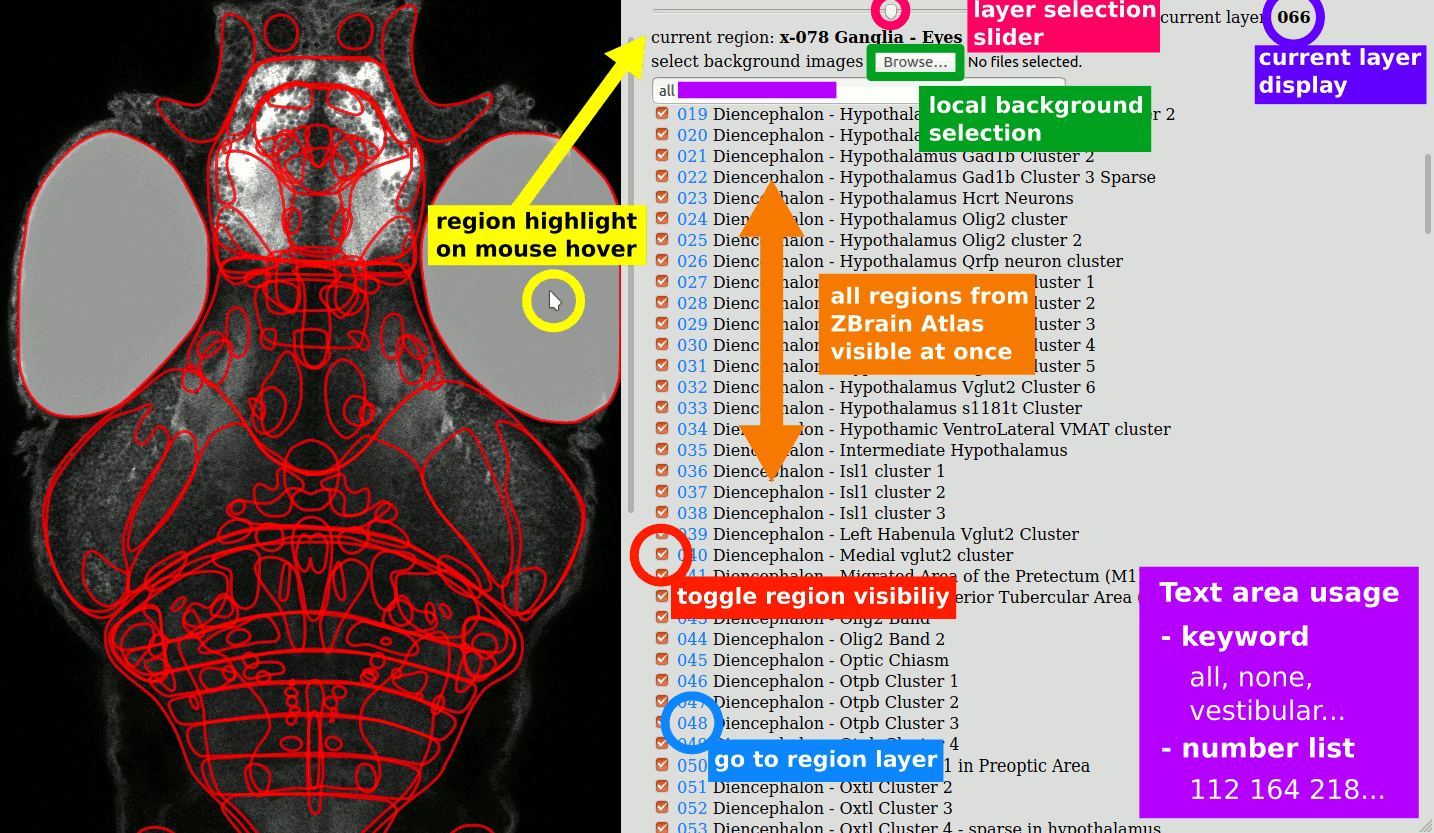
\includegraphics[width=\textwidth]{./files/LJPzebrain_screenshot.png}
\caption{Annotated screenshot showing all the features of the LJP zebrain viewer.}
\end{figure}

Les outils évoqués ci-dessus permettent d'explorer une grande variété de données mises en commun mais sont assez complexes et nécessitent une bonne connaissance préalable de l'anatomie du cerveau. Ils sont difficiles à prendre en main et ne permettent pas de travailler avec des données locales. J'ai donc conçu un prototype à ambition pédagogique destiné aux débutants en imagerie de cerveau de larve de poisson zèbre ou pour dégrossir rapidement des données locales.

Le \href{https://github.com/LJPZebra/zebrain}{LJP zebrain} permet de charger une liste d'images locales correspondant au cerveau transformé dans l'espace de référence ZBrain et d'explorer les régions par un simple survol de souris. Cela facilite notamment l'exploration des cartes de phase.





% outils généralistes
% 3DSlicer
% CMTK
% Ants
% ImageJ



% outils de productivité
% Zotero
% Inkscape
% GIMP
% git


\chapter{Détail de calcul}\label{calculdetail}

Détail du calcul pour le déphasage d'un sinus après convolution par une exponentielle décroissante. L'idée consiste à effectuer deux fois une intégration par partie.

$$
\text{(intégration par partie)} \quad \int_a^buv' = \Big[uv\Big]_a^b - \int_a^b u'v
$$

$$ A(t) = \sin(\omega t) $$
$$ K(t) = \frac{1}{\tau}\exp\left(-\frac{t}{\tau}\right)H(t) $$
$$ F(t) = (A\circledast K)(t) $$ 
$$
F(t) = \int_{-\infty}^\infty\sin(\omega(t-t'))\frac{1}{\tau}\exp\left(-\frac{t'}{\tau}\right)H(t')\mathrm{d}t'
$$
$$
F(t) = \int_{0}^\infty\underbrace{\sin\bigg(\omega(t-t')\bigg)}_u\underbrace{\frac{1}{\tau}\exp\left(-\frac{t'}{\tau}\right)}_{v'}\mathrm{d}t'
$$
\begin{multline}
F(t) = \left[\sin(\omega(t-t'))\left(-\exp\left(-\frac{t'}{\tau}\right)\right)\right]_0^\infty \\ -
\int_{0}^\infty\underbrace{-\omega\cos\bigg(\omega(t-t')\bigg)}_u\underbrace{\left(-\exp\left(-\frac{t'}{\tau}\right)\right)}_{v'}\mathrm{d}t'
\end{multline}
\begin{multline}
F(t) = \sin(\omega t) -
\Bigg(\left[\omega\cos(\omega(t-t'))\left(-\tau\exp\left(-\frac{t'}{\tau}\right)\right)\right]_0^\infty \\ -
\int_0^\infty\omega^2\sin(\omega(t-t'))\left(-\tau\exp\left(-\frac{t'}{\tau}\right)\right)\mathrm{d}t' \Bigg)
\end{multline}
$$
F(t) = \sin(\omega t) - \omega\tau\cos(\omega t) - \omega^2\tau^2\int_0^\infty\sin(\omega(t-t')) \frac{1}{\tau}\exp\left(-\frac{t'}{\tau}\right)\mathrm{d}t'
$$
Donc
$$
(1+\omega^2\tau^2)\int_0^\infty\sin(\omega(t-t')) \frac{1}{\tau}\exp\left(-\frac{t'}{\tau}\right)\mathrm{d}t' = \sin(\omega t) - \omega\tau\cos(\omega t)
$$
Soit
$$
F(t) = \frac{\sin(\omega t)}{1+\omega^2\tau^2} - \frac{\omega\tau\cos(\omega t)}{1+\omega^2\tau^2}
$$
$$ \text{(sinus d'une somme)}  \quad  \sin(a+b) = \sin a\cos b + \cos a\sin b $$
$$
\sin(\omega t+\varphi) = \sin(\omega t)\underbrace{\frac{1}{1+\omega^2\tau^2}}_{\cos\varphi} + \cos(\omega t)\underbrace{\frac{-\omega\tau}{1+\omega^2\tau^2}}_{\sin\varphi}
$$
$$ \tan\varphi = \frac{\sin\varphi}{\cos\varphi} = -\omega\tau $$
$$ \varphi = \mathrm{atan}(-\omega\tau) $$
$$ F(t) = \sin(\omega t + \varphi) $$

Donc la convolution d'un sinus de pulsation $\omega$ par un noyau en exponentielle décroissante de temps caractéristique $\tau$ résulte en un déphasage négatif (retard temporel) de $ \varphi = \mathrm{atan}(-\omega\tau) $.